\documentclass{article}
\usepackage[a4paper, margin=1.5cm]{geometry}
\usepackage{amsmath, amsfonts}
\usepackage{tasks}

\usepackage{tikz, pgfplots}
\usepgfmodule{nonlineartransformations}
\pgfplotsset{
  compat=1.16,
  xyplane/.style = {
    width=5cm, height=5cm,
    anchor=center,
    axis equal,
    axis x line=middle,
    axis y line=middle,
    axis line style={stealth-stealth, very thick},
    samples=10,
    xmin=-2.5, xmax=2.5,
    ymin=-2.5, ymax=2.5,
    xtick={-2,-1,...,2},
    ytick={-2,-1,...,2},
    grid=major,
    major grid style={black!30},
    xticklabels={,},
    yticklabels={,},
  },
}

\newcommand{\LTplane}[4]{
  \begin{center}
    \begin{tikzpicture}
      \pgftransformcm{#1}{#2}{#3}{#4}{\pgfpoint{0}{0}}
      \begin{axis}[
          xyplane,
        ]
        \draw[very thick, fill=red!25] (0,0) rectangle (1,1);
        \draw[very thick, fill=blue!25] (0,0) rectangle (-1,-1);
        \draw[very thick, fill=green!25] (0,0) rectangle (-1,1);
        \draw[very thick, fill=orange!25] (0,0) rectangle (1,-1);
      \end{axis}
    \end{tikzpicture}
  \end{center}
}

\makeatletter
\def\trigtrans{%
  \pgfmathsetmacro{\myX}{\pgf@x + 4*sin(4*\pgf@y) }
  \pgfmathsetmacro{\myY}{\pgf@y}
  \setlength{\pgf@x}{\myX pt}
  \setlength{\pgf@y}{\myY pt}
}
\def\parabtrans{%
  \pgfmathsetmacro{\myX}{\pgf@x + 0.002*\pgf@y^2}
  \pgfmathsetmacro{\myY}{\pgf@y - 0.002*\pgf@x^2}
  \setlength{\pgf@x}{\myX pt}
  \setlength{\pgf@y}{\myY pt}
}
\makeatother

\title{Gauging student's intuition and understanding of linear algebra}
\author{Peleg Sapir}

\begin{document}
\maketitle
\section{Vectors}
\subsection{Orthogonal vectors}
Briefly explain the following fact: given a vector $\vec{v}\in\mathbb{R}^{2},\ \vec{v}=\begin{pmatrix}x\\y\end{pmatrix}$, rotating it by $\pm\frac{\pi}{2}$ yields the vectors $\vec{u}=\begin{pmatrix} -y\\x\end{pmatrix}$ and $\vec{w}=\begin{pmatrix} y\\-x\end{pmatrix}$.
\subsection{Basis sets}
Briefly explain the \textit{Gram-Schmidt} process in geometric terms.

\section{Linear transformations}
\subsection{Geometry of linear transformations}
The following is a geomteric visualization of the space
$\mathbb{R}^{2}$, highlighting four unit squares, each between the origin and
a point from $(1,1),\ (-1,1),\ (-1,-1),\ (1,-1)$ (colored in red, green, blue,
and orange - respectively):

\LTplane{1}{0}{0}{1}

Which of the following \textit{images} of $\mathbb{R}^{2}$ is a
result of a linear transformation applied on it, and which isn't?

\begin{tasks}[label-width=1.5em](3)
  \task \LTplane{1}{0}{0.5}{1}
  \task \LTplane{0}{-1}{1}{0}
  \task \LTplane{-1}{0}{0}{1}
  \task
  \begin{center}
    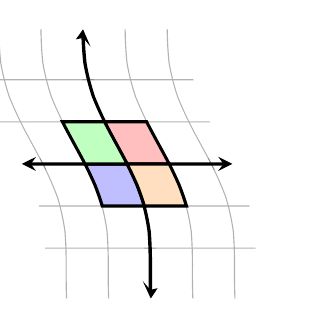
\begin{tikzpicture}
      \pgftransformnonlinear{\trigtrans}
      \begin{axis}[
          xyplane,
        ]
        \draw[very thick, fill=red!25] (0,0) rectangle (1,1);
        \draw[very thick, fill=blue!25] (0,0) rectangle (-1,-1);
        \draw[very thick, fill=green!25] (0,0) rectangle (-1,1);
        \draw[very thick, fill=orange!25] (0,0) rectangle (1,-1);
      \end{axis}
    \end{tikzpicture}
  \end{center}
  \task \LTplane{-1}{0}{0}{1}
  \task \LTplane{0.707}{0.4}{-0.707}{0.4}
  \task
  \begin{center}
    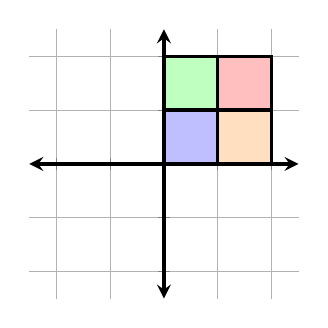
\begin{tikzpicture}
      \begin{axis}[
          xyplane,
        ]
        \draw[very thick, fill=red!25] (1,1) rectangle (2,2);
        \draw[very thick, fill=blue!25] (1,1) rectangle (0,0);
        \draw[very thick, fill=green!25] (1,1) rectangle (0,2);
        \draw[very thick, fill=orange!25] (1,1) rectangle (2,0);
      \end{axis}
    \end{tikzpicture}
  \end{center}

  \task
  \begin{center}
    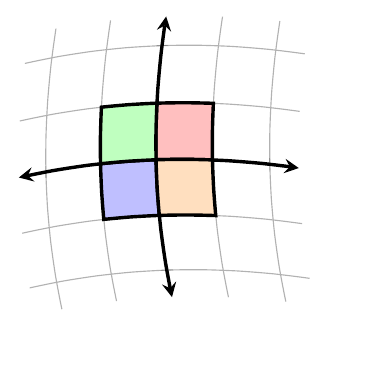
\begin{tikzpicture}
      \pgftransformnonlinear{\parabtrans}
      \begin{axis}[
          xyplane,
        ]
        \draw[very thick, fill=red!25] (0,0) rectangle (1,1);
        \draw[very thick, fill=blue!25] (0,0) rectangle (-1,-1);
        \draw[very thick, fill=green!25] (0,0) rectangle (-1,1);
        \draw[very thick, fill=orange!25] (0,0) rectangle (1,-1);
      \end{axis}
    \end{tikzpicture}
  \end{center}

  \task \LTplane{1}{0}{0}{0.75}
\end{tasks}

\section{Matrices}
\subsection{Non-commutativity of matrix multiplication}
Explain in a simple and concise manner why matrix-matrix products are
usually not commutative.

\subsection{Matrix of a composite transformation}
Use a product of several matrices to find the matrix representation of the following transformation $T:\mathbf{R}^{2}\to\mathbf{R}^{2}$: reflection across any line that goes through the origin. \textbf{Hint}: you can define the line using its angle to either the $x$-axis or the $y$-axis.

\subsection{Matrix operations}
Give a concise geomteric explanation of the operation(s) made by each
of the following matrices:

\begin{tasks}[label-width=1.5em](3)
  \task $
  \begin{pmatrix} 2 & 0 \\ 0 & 1 \\
  \end{pmatrix} $

  \task $
  \begin{pmatrix} 0 & 1 \\ 1 & 0 \\
  \end{pmatrix} $

  \task $
  \begin{pmatrix} 0 & -1 \\ 1 & 0 \\
  \end{pmatrix} $

  \task $
  \begin{pmatrix} 1 & 1 \\ 0 & 0 \\
  \end{pmatrix} $

  \task $
  \begin{pmatrix} -1 & 0 \\ 0 & 1 \\
  \end{pmatrix} $

  \task $
  \begin{pmatrix} 1 & \frac{1}{2} \\ 0 & 1 \\
  \end{pmatrix} $

  \task $
  \begin{pmatrix} 1 & 0 \\ 0 & 2
  \end{pmatrix} \cdot
  \frac{1}{\sqrt{2}}
  \begin{pmatrix} 1 & -1 \\ 1 & 1
  \end{pmatrix} $

  \task $
  \frac{1}{\sqrt{2}}
  \begin{pmatrix} 1 & -1 \\ 1 & 1
  \end{pmatrix} \cdot
  \begin{pmatrix} 1 & 0 \\ 0 & 2
  \end{pmatrix} $

  \task $
  \begin{pmatrix} 1 & 0 & 0 \\ 0 & 0 & -1 \\ 0 & 1 & 0
  \end{pmatrix} $
\end{tasks}

\subsection{The determinant}
Without calculating directly, what is the expected determinant of each
of the following matrices?

\begin{tasks}[label-width=1.5em](3)
  \task $
  \begin{pmatrix} 2 & 0 \\ 1 & 1
  \end{pmatrix}$

  \task $
  \begin{pmatrix} 0 & 1 & 0 \\ 1 & 0 & 0 \\ 0 & 0 & 1
  \end{pmatrix}$

  \task $
  \begin{pmatrix} \cos(\theta) & 0 & \sin(\theta) \\ 0 & 1 & 0
    \\ \sin(\theta) & 0 & \cos(\theta)
  \end{pmatrix}$

  \task $
  \begin{pmatrix} 2 & 3 & 1 \\ 0 & 0 & 0 \\ 1 & -5 & 7
  \end{pmatrix}$

  \task $
  \begin{pmatrix}
    3 & 1 & 7  & 2\\
    3 & 2 & 2  & 4\\
    5 & 4 & 5  & 8\\
    1 & 0 & -1 & 0 \\
  \end{pmatrix}$

  \task $
  \begin{pmatrix}
    7 & 7 & 4 & 4 \\
    5 & 6 & 0 & -1 \\
    2 & 1 & 4 & 5 \\
    -2 & 5 & 8 & 1 \\
  \end{pmatrix}$
\end{tasks}

\section{Eigenvalues and eigenvectors}
Without calculating directly, what are the expected eigenvectors (and
corresponding eigenvalues) of each of the following matrices? Use a
formal calculation to see if you were correct.

\begin{tasks}[label-width=1.5em](3)
  \task $
  \begin{pmatrix} s & 0 \\ 0 & 1
  \end{pmatrix},\ 0\neq s \in\mathbb{R}$

  \task $
  \begin{pmatrix} 1 & k \\ 0 & 1
  \end{pmatrix},\ 0\neq k \in\mathbb{R}$

  \task $
  \frac{1}{2}
  \begin{pmatrix} \sqrt{3} & 1 \\ 1 & \sqrt{3}
  \end{pmatrix}$

  \task $
  \begin{pmatrix} \cos(x) & -\sin(x) \\ \sin(x) & \cos(x)
  \end{pmatrix}$

  \task $
  \begin{pmatrix} \cos(x) & -\sin(x) & 0 \\ \sin(x) & \cos(x) & 0 \\ 0 & 0 & 1
  \end{pmatrix}$
\end{tasks}

\end{document}
